\documentclass[11pt]{article}
%---- defitions ----
\def\Author{Andreas Bock, bock@andreasbock.dk\\
Johan Astborg, joastbg@gmail.com\\\\
Supervisors:\\
Jost Berthold, jb.diku@gmail.com\\
Sinan Gabel, sinan.gabel@gmail.com
}
%\def\Title{\bf Project Synopsis\\ HQL - \textsc{Hiperfit} Quant Library}
\def\Title{\bf HQL - \textsc{Hiperfit} Quant Library\\ {\Large Project Synopsis}}
% <Add more defitions here>
%-------------------

%---- packages ----
\usepackage[]{amsmath}
\usepackage[english]{babel}
\usepackage[utf8]{inputenc}
\usepackage{graphicx}
\usepackage{moreverb}
\usepackage{hyperref}
\usepackage{color}
\usepackage{listings}

%---- settings ----
% Comments
\newcommand{\comm}[2]{{\sf \(\spadesuit\){\bf #1: }{\rm \sf #2}\(\spadesuit\)}}
\newcommand{\mcomm}[2]{\marginpar{\scriptsize \comm{#1}{#2}}}
\newcommand{\ab}[1]{\mcomm{AB}{#1}}
\newcommand{\ja}[1]{\mcomm{JA}{#1}}

\topmargin=-1.1in % start text higher on page
\textheight=695pt
\usepackage[T1]{fontenc} % font
\setlength{\parindent}{0in}
\definecolor{lightgray}{rgb}{0.9,0.9,0.9}

\newenvironment{filecode}[1][]
{\minipage{\linewidth}
\lstset{basicstyle=\ttfamily\footnotesize,frame=single,
numberstyle=\small\color{black},keywordstyle=\color{black},commentstyle=\color{black},stringstyle=\color{black},tabsize=2,backgroundcolor=\color{lightgray},language=Haskell,#1}}
{\endminipage}
%-------------------

\begin{document}
\title{\Title}
\author{\Author}
\date{\today}
\maketitle

\begin{abstract}

% Something about how pricing is done now, and what we will do

\end{abstract}

\section*{Introduction}

Our everyday lives becoming increasingly dependent on IT, and as a result, software
errors are manifold. The financial sector has a particular low tolerance, as erroneous
software may have dire consequences in the form of massive monetary loss.
Human brokers are replaced by computer systems, and traders are now joined by
colocated machines that perform high-frequency trading using predefined and backtested algorithms.\\

\begin{comment}
Backtesting is a method where historical data is used to evaluate the performance of said
trading algorithm. This includes computing the present value of a portfolio to assess whether
the trader's funds could be utilized more efficiently elsewhere.
However, an otherwise feasible trading model could wreak havoc on markets because of a software error
which stresses the need for code correctness for both the algorithms and our assesment of them.\\
\end{comment}

A language that, by design, allows us to discover a large portion of software errors in 
the compilation phase is therefore preferable in the financial domain. 

Our project will deliver a proof of concept library for pricing financial contracts.
We will implement it using the pure functional programming language Haskell which features
many attractive properties that steer us toward producing safe and correct code.\\

The library is intended to be used for the following purposes:
%\ab{This shouldn't be included, this is the learning goals/problem statement}.
\begin{itemize}
\item Numerical valuation of financial contracts with closed-form solutions
\item Simulations and backtesting
\item Explore and develop new contract types from existing ones
\item Research and education
\end{itemize}

By designing and building our software using Haskell, we hope to eliminate some
of the unnecessary risk in financial modelling and this project will investigate these possibilities.\\

\begin{comment}
What if, many of the errors in software could be discovered by the compiler through clever
usage of types and much stricter rules for conversion of such using casting. We will
try to reach a proof of concept level using a pure functional programming language called Haskell \cite{Haskell},
 where many desirable constructs for building robust and safe software is implemented.\\

By designing and building our software using Haskell, we hope to eliminate some
of the unnecessary risk in financial modelling, and this project will investigate these possibilities.\\

%Backtesting is a method used for testing trading algorithms on historical data
%to be able to evaluate their performance in terms of returns, volatility etc.

% Algorithms
These tools may help increase competitiveness and profits in unexploited areas, but emphasize the
importance of correct and efficient code.

Automated algorithmic trading systems are considered to have lower operational risk due to minimal human interaction, but require software correctness to work. 
An otherwise feasible trading model could wreak havoc on markets because of a software error.

% Safeguards are also compromised
Further, brokerages and exchanges attempt to lower operational risk by implementing
safeguards, known as pre-trade risk rules, to prevent human error to affect markets (e.g. fat-fingering
trades\footnote{Human error causing larges trades to be made that create sudden
imbalances in the markets.}). Albeit thoroughly tested, bugs are ubiquitous and these
safeguards may be just as prone to them. 

% Legislation, cite new Danish regulations?
The financial crisis of 2008 also caused legislators to take a more conservative
stance on risk, as the collapse on Lehman Brothers reverberated throughout
the world's economies.
Consequently, financial institutions' risk management tools must become more
sophisticated, putting stress on the quality of the software.

The library is intended to be used for the following purposes:\ab{This shouldn't be included, this is the learning goals/problem statement}.
\begin{itemize}
\item Numerical valuation of financial contracts with closed-form solutions
\item Simulations and backtesting
\item Explore and develop new contract types from existing ones
\item Research and education
\end{itemize}

\end{comment}

\section*{Problem Statement}

In this project we will design the software architecture for a Haskell library for quantitative finance.
The desired functionality is modeled after an existing Mathematica library {\tt DerivativesExpert}, which
we will re-engineer using Haskell.
The main objective is to use the Haskell programming language for design and architecture and reach a proof-of-concept level.
The project is conducted within the HIPERFIT research center.

\section*{Elaboration}

% TODO Mention Quantlib
In finance, a portfolio is a number of positions such as long or short trades in equities, bonds and other
types of financial instruments. The present value of such a collection can be computed through
discounting to reflect the theoretical value they would have if they existed today. This allows
investors to evaluate if their resources could yield higher returns elsewhere.
Financial instruments are priced differently, some using closed-form functions and
others relying on stochastic simulation. In this project, we'll mainly work with closed-form functions for bonds and
the time value of money.\\

Functional languages lend themselves well to the domain of finance due
to several reasons. Firstly, functions are first-class citizens, and programs are constructed
from functions entirely. Because of the mathematical nature of finance, a functional
programming language is preferable and makes it easier to write and test mathematical expressions.\\

Further, Haskell is a pure language meaning that a function will always return the same value
if given the same input. This makes it ideal for
financial computations where we want to be certain our computations are not changed by some
global state. In Haskell, the programmer is always aware of whether the constructs used will affect
state or note, because of the clear distinction made between pure functions and  monads that induce state \footnote{the \texttt{I/O} monad}.\\

Combining Haskell's purity with its modularity, we can also allow for users to `glue`
together functions without the worry that, for instance, the first function call has changed
a value through a pointer. Function composition in this manner does not mean we
take a penalty performance-wise, since the non-strictness of the language  means that
we only evaluate the things we need.\\

Additionally, Haskell is a statically typed language with type inference. As such, 
types and type classes make up a large portion of the language design. Statically typed languages have the
advantage of discovering many errors at compile time, and the type class system enables us to overload
functionality in our programs based on our types.
This is a very desirable feature, as we want our financial
products to have the same API (e.g. a function \texttt{presentValue} should return the
present value regardless of the product type).\\

%% More technical details
%As part of the input to the project, we have access to existing test-cases written in Mathematica code.
%These will be ported to QuickCheck \cite{QuickCheck}, which is a combinator library for generating test cases in Haskell.

We will now exemplify our use of Haskell's type system in modelling financial contracts.
As a starting point we ask ourselves what functionality we wish to have when we modelling
any financial instrument.
Haskell's type classes can be used to define interfaces for our financial products:

\begin{center}
\tt
\begin{tabular}{lll}
class & Instrument i where\\
      &\hspace{-1cm} pv       :: i -> DiscountFunction -> Payment\\
      &\hspace{-1cm} cashflow :: i -> CashFlow\\
\end{tabular}
\end{center}

such that instances of {\tt Instrument} must implement {\tt pv} and {\tt cashflow}, each
computing the present value and cash flow (series of future payments) respectively.

Now turning to specific instruments, a common bond can be represented by a
Haskell data type:

\begin{center}
\tt
\begin{tabular}{lll}
data & CommonBond = CommonBond \{\\
      &\hspace{-1cm} principal :: Payment,\\
      &\hspace{-1cm} ts :: TermStructure\\
      &\hspace{-1cm}\}
\end{tabular}
\end{center}

As a {\tt CommonBond} is indeed a finanicial instrument we may make it an instance of
the {\tt Instrument} class and define its functions based on appropriate mathematical
formulas.

Haskell's type hierarchy allows us to define a new type class that more precisely
defines the desired interface for bonds:

\begin{center}
\tt
\begin{tabular}{lll}
class & Instrument b => Bond b where\\
      &\hspace{-1cm} principal :: b -> Payment\\
      &\hspace{-1cm} coupon    :: b -> Payment\\
      &\hspace{-1cm} maturity  :: b -> Date\\
      &\hspace{-1cm} discount  :: b -> DiscountFunction\\
      ...
\end{tabular}
\end{center}

We may continue to define new classes in this manner, forming a tree-like
structure of the classes. We seek to identify this inheritance relations among
financial products and model them in Haskell through the hierarchical structure
of the class system.\\

Finally, functional languages can easily preserve the inherent parallelism of computations 
making them ideal for performance-critical tasks such as pricing financial products or
computing risk.\\

In summary, our focus will be on exploring how Haskell's language features can be used
to ensure safe and correct code, without compromising a good extendable software architecture.

\section*{Learning Goals}

Learning goals and objectives:

\begin{enumerate}
\item The student will be able to design and implement medium to large scale software systems in a functional language. % arch
\item The students will be able to describe the concepts of financial valuation and its relevance to portfolio management. % finance
\item The students will be able to develop a sustainable and extendable prototype Haskell library for pricing common financial products. % concrete result
\item The students will be able to analyse the functionality of existing software and re-engineer it in a functional language.
\end{enumerate}

\section*{Limitations}

% 1) Not a fully-fledged library like DE or Quantlib
We will not expect to produce a fully-fledged library like {\tt DerivativesExpert} or Quantlib\cite{Ame2003}.
% 2) Benchmarking or comparisons (?)
Secondly, and partly due to the point above, we will not perform an in-depth survey
comparing the result of our project with similar ones such as the aforemetioned libraries.

The lack of a symbolic computation engine in our project, which is part of Mathematica, may limit us
in terms of flaoting point precision. If this has any practical significance remains to be evaluated.

% 3)

The project is mainly limited by time, a constraint derived from the project course 
format (one block lasting approximately 9 weeks).
The scope has been narrowed to fit the size of the project, and will mainly include
pricing functionality for different bond types specified in the {\tt DerivativesExpert} package.




\section*{Possible additions}

There are a number of day count conventions in the financial world, so a
calendar library that supports these peculiarities would be valuable for the precision
of our pricing methods.\\

% More technical details
%Another possible addition would be to port the have access to existing test-cases written in Mathematica code.
%These will be ported to QuickCheck \cite{QuickCheck}, which is a combinator library for generating test cases in Haskell.

A natural development of the project is to introduce a combinator library for composing contracts
from atomic constructs, as proposed by Peyton Jones et al. \cite{Pjes2000}.\\ \ab{This needs to be elaborated}\\

Another possible addition to the library could be a domain-specific language (DSL) for modelling \emph{over-the-counter} (OTC) contracts, i.e. where two parties agree to trade a product given some conditions outside regular exchanges.

\section*{Schedule}

%% Use milestones here instead?

Below is our approximate schedule over the course of the project:

\begin{figure}[h!]
\begin{center}
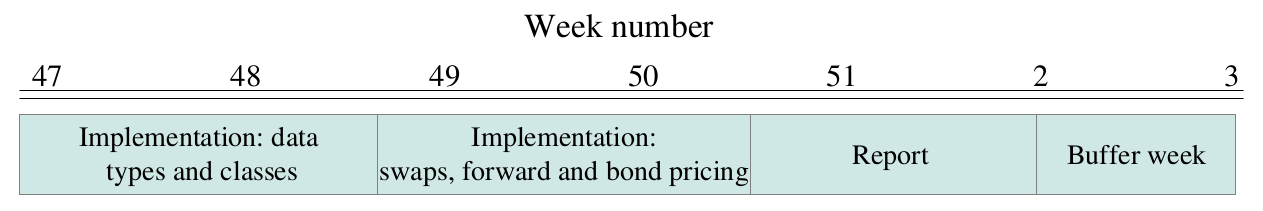
\includegraphics[bb = 0 0 1302 348, scale=0.275]{schedule.png}
\end{center}
\end{figure}

% REFERENCES
\bibliographystyle{abbrv}
%\addcontentsline{toc}{section}{References}
\bibliography{hql}

\end{document}
